\documentclass[informe.tex]{subfiles}
\begin{document}

\textbf{Función de transformación}\newline

La función de transformación a un filtro pasa alto (HP) no normalizado, $T_{HP}(s)$, hacia un filtro pasa bajo normalizado (LP), $T_{LP}(s)$, es:
	\begin{equation}
		\label{eqn:hp:lp1}	
		S=\frac{\omega_p}{s}
	\end{equation}
o bien, siendo $S=j\Omega$ y $s=j\omega$, con la siguiente función de transformación
	\begin{equation}
		\label{eqn:hp:lp2}	
		\Omega=\frac{-\omega_p}{\omega}
	\end{equation}\newline
		
\textbf{Procedimiento de resolución de filtros paso alto.}\newline

1- Al conjunto de requerimientos dados de un filtro pasa alto:
	\begin{center}			 
				($A_{max}$, $\omega_p$, $A_{min}$, $\omega_s$)
	\end{center}
	donde,
	\begin{tabbing}
		\phantom{$D_{n50}\ $}\= \kill
		$A_{max}$\> , Atenuación máxima dada en la frecuencia en la banda de paso, $\omega_p$ \\
		$\omega_p$\> , Frecuencia dada en la banda de paso.\\
		$A_{min}$\> , Atenuación mínima dada en la frecuencia en la banda de rechazo, $\omega_s$. \\
		$\omega_s$\> , Frecuencia dada en la banda de rechazo.				
	\end{tabbing}
	
	
Estos requerimientos se transforman con la expresión dada en Ec. \ref{eqn:hp:lp1} 	a los requerimientos equivalentes del filtro paso bajo normalizado
    \begin{center}
				($A_{max}$, $1$, $A_{min}$, $\Omega_s=\omega_p/\omega_s$)
    \end{center}				
	
		\begin{figure}[h]
		\centering
		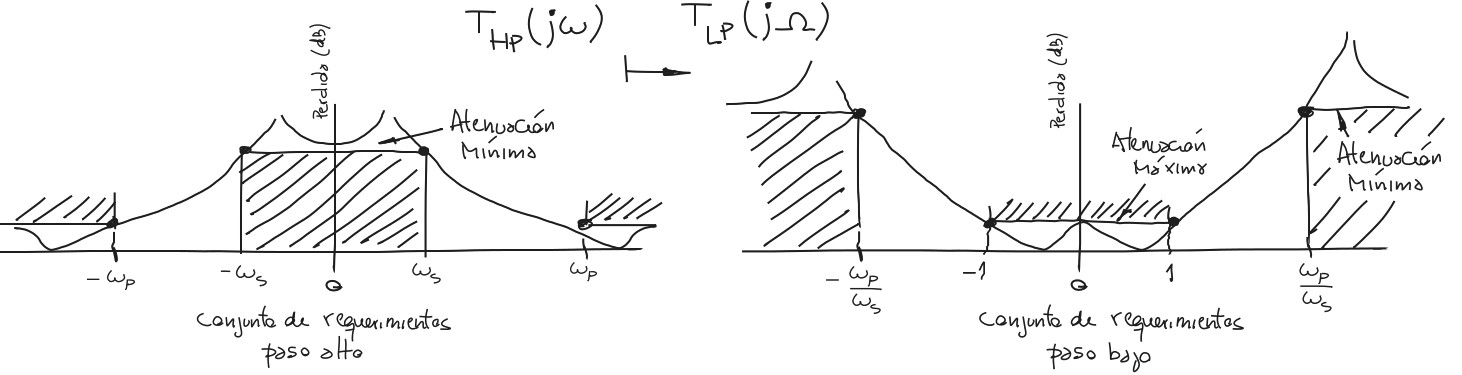
\includegraphics[scale=1.1]{transformacion_2_hp.jpg}
		\caption{Funciones de atenuación. A la izquierda el filtro pasa alto. A la derecha el filtro pasa bajo}
		\label{fig:transformacion:hp:func_att}
		\end{figure}	
		
		\begin{figure}[h]
		\centering
		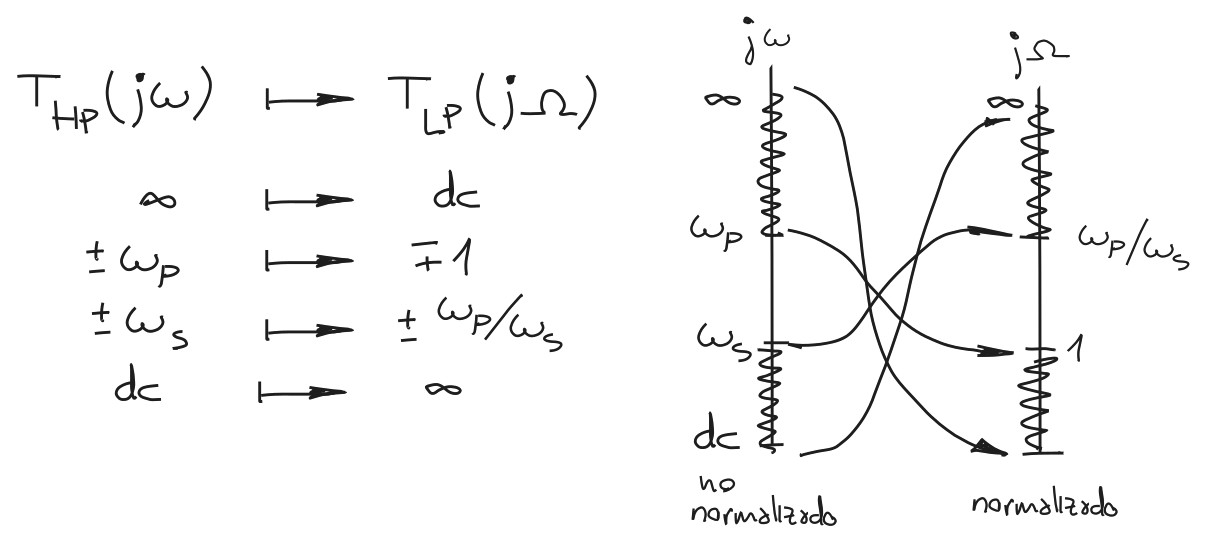
\includegraphics[scale=0.8]{transformacion_3_hp.jpg}
		\caption{Relaciones entre las frecuencias de un filtro pasa alto y un filtro pasa bajo.}
		\label{fig:transformacion:hp:relaciones}
		\end{figure}	
			
2- Seguido, se determina la función que aproxime los requerimientos pasa bajos, según la aplicación requerida por el filtro ( Butterworth, Chebyshev o Bessel ).\newline\newline			
3- Por último, la función $T_{LP}(S)$ se transforma a la función $T_{HP}(s)$ con la Ec. Ec. \ref{eqn:hp:lp1}, quedando.
				$$T_{HP}(s)= \left.  T_{LP(S)} \right|_{S=\omega_p/s}$$
				
%%  
\textbf{Ejemplo con Matlab:} Creando una función de Matlab que permita realizar la transformación de paso alto a paso bajo.\newline  

\lstinputlisting[language=Matlab, frame=single, extendedchars=true]{./src_matlab/mi_lp2hp.m}  				
				
\end{document}	